%%%%%%%%%%%%%%%%%%%%%%%%%%%%%%%%%%%%%%%%%%%%%%%%%%%
%% P3: Phenomenology of Particle Physics                         
%%
%% Author:  André Rubbia                   		 
%%
%% Figure 13.12 Cross-section distributions for the reaction $e^+e^-\rightarrow \gamma\gamma$.
%%
%% This work is licensed under the Creative Commons Attribution 4.0 International License. 
%% To view a copy of this license, visit http://creativecommons.org/licenses/by/4.0/ or 
%% send a letter to Creative Commons, PO Box 1866, Mountain View, CA 94042, USA.
%%
%%%%%%%%%%%%%%%%%%%%%%%%%%%%%%%%%%%%%%%%%%%%%%%%%%%

\documentclass[a4paper,10pt]{article}

\usepackage[T1]{fontenc}
\usepackage[utf8]{inputenc}
\usepackage{lmodern}
\usepackage[labelfont=bf]{caption}
\usepackage{upgreek}

\usepackage{tikz}
\usepackage{pgfplots}
\pgfplotsset{compat=1.17}
\usepgfplotslibrary{ternary}
\usepgfplotslibrary{fillbetween}
\usepgfplotslibrary{external}

\usepackage{braket}

\def\d{\mathrm{d}}

\pgfkeys{/pgf/number format/.cd,1000 sep={}}

\begin{document}

%%%%%%%%%%%%%%%%% FIGURE %%%%%%%%%%%%%%%%%%%%%%%%%%%%%%%%%%
\begin{figure}[htb]
\begin{center}
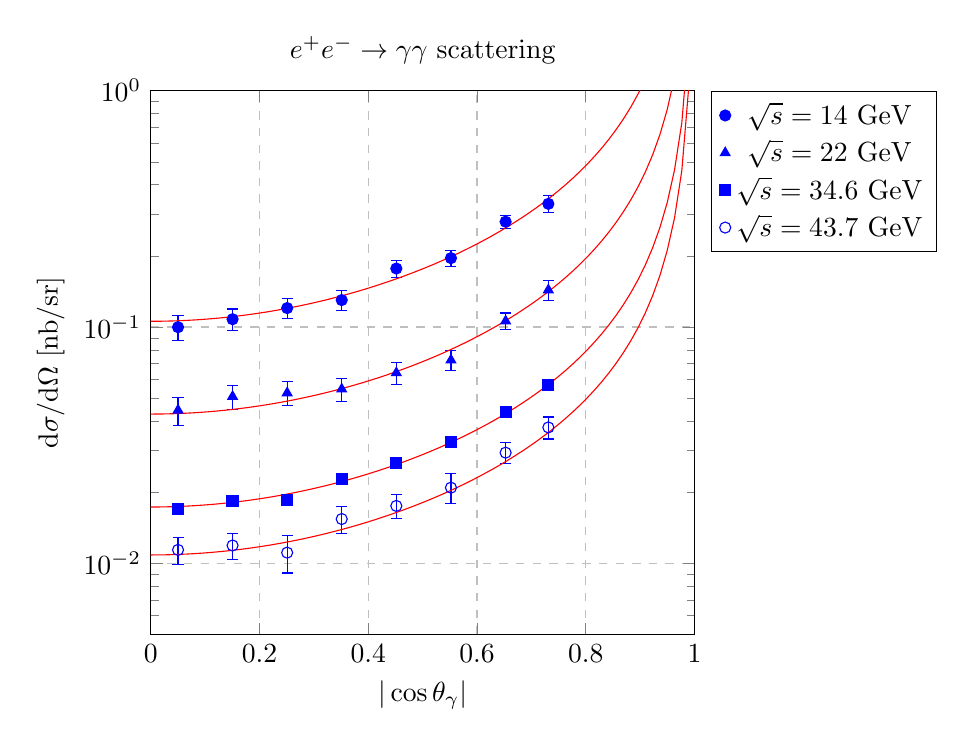
\begin{tikzpicture}[scale=1.]
\begin{semilogyaxis}[
    width=0.7\textwidth,
    height=0.7\textwidth,
    title={$e^+e^-\rightarrow \gamma\gamma$ scattering},
    xlabel={$\vert\cos\theta_\gamma\vert$},
    ylabel={${\d\sigma}/{\d\Omega }$ [nb/sr]},
    xmin=0, xmax=1,
    ymin=0.005, ymax=1,
%    xtick={0,20,40,60,80,100,120,140,160},
%    tick={1e0,1e1,1e2,1e3,1e4,1e5,1e6,1e7},
	legend style={legend pos = outer north east},
    	ymajorgrids=true,
    	xmajorgrids=true,
    grid style=dashed,
]

%% JADE $\sqrt{s}=14$~GeV
\addplot[
    color=blue,
    only marks,
    error bars/.cd,
    y dir=both, y explicit
    ]
    coordinates {
(0.0502,0.09983)+-(0,0.01178)
(0.1505,0.10791)+-(0,0.01126)
(0.2509,0.12026)+-(0,0.01198)
(0.3512,0.13002)+-(0,0.01243)
(0.4516,0.17681)+-(0,0.01486)
(0.5521,0.1957)+-(0,0.0154)
(0.6526,0.279)+-(0,0.01834)
(0.7312,0.33204)+-(0,0.02665)
};

%% JADE $\sqrt{s}=22$~GeV
\addplot[
    color=blue,
    only marks,
    mark = triangle*,
    error bars/.cd,
    y dir=both, y explicit
    ]
    coordinates {
(0.0502,0.04446)+-(0,0.00599)
(0.1505,0.05079)+-(0,0.0059)
(0.2509,0.0526)+-(0,0.00608)
(0.3512,0.0546)+-(0,0.00612)
(0.4516,0.06397)+-(0,0.00687)
(0.5521,0.07243)+-(0,0.00703)
(0.6526,0.10595)+-(0,0.00864)
(0.7312,0.14343)+-(0,0.01363)
};

%% JADE $\sqrt{s}=34.6$~GeV
\addplot[
    color=blue,
    only marks,
    mark = square*,
    error bars/.cd,
    y dir=both, y explicit
    ]
    coordinates {
(0.0502,0.01694)+-(0,0.00071)
(0.1505,0.01842)+-(0,0.00069)
(0.2509,0.01859)+-(0,0.00059)
(0.3512,0.02282)+-(0,0.00077)
(0.4516,0.02668)+-(0,0.00085)
(0.5521,0.03266)+-(0,0.00092)
(0.6526,0.04363)+-(0,0.00107)
(0.7312,0.05664)+-(0,0.00162)
};

%% JADE $\sqrt{s}=43.7$~GeV
\addplot[
    color=blue,
    only marks,
    mark = o,
    error bars/.cd,
    y dir=both, y explicit
    ]
    coordinates {
(0.0502,0.0114)+-(0,0.0015)
(0.1505,0.0119)+-(0,0.0015)
(0.2509,0.0111)+-(0,0.002)
(0.3512,0.0154)+-(0,0.002)
(0.4516,0.0175)+-(0,0.002)
(0.5521,0.0209)+-(0,0.003)
(0.6526,0.0294)+-(0,0.003)
(0.7312,0.0376)+-(0,0.004)
};

       \addplot [red,domain=0:0.99, samples=75] {1e6*(1/137^2)*0.389/196*(1+x^2)/(1-x^2)};
       \addplot [red,domain=0:0.99, samples=75] {1e6*(1/137^2)*0.389/484*(1+x^2)/(1-x^2)};
       \addplot [red,domain=0:0.99, samples=75] {1e6*(1/137^2)*0.389/1197*(1+x^2)/(1-x^2)};
       \addplot [red,domain=0:0.99, samples=75] {1e6*(1/137^2)*0.389/1910*(1+x^2)/(1-x^2)};

    \legend{ $\sqrt{s}=14$~GeV,
      $\sqrt{s}=22$~GeV,
       $\sqrt{s}=34.6$~GeV,
      $\sqrt{s}=43.7$~GeV
	}
\end{semilogyaxis}
\end{tikzpicture}
\caption{Cross-section distributions for the reaction $e^+e^-\rightarrow \gamma\gamma$ measured
by JADE at PETRA: differential cross-sections at $\sqrt{s} = 14, 22, 34.6$ and 43.7~GeV compared
to QED predictions (straight lines).}
\end{center}
\end{figure}
%%%%%%%%%%%%%%%%% END FIGURE %%%%%%%%%%%%%%%%%%%%%%%%%%%%%%
%

\end{document}
